\chapter{Introduction}
To establish the framework in which this thesis has been developed, a general overview of the MariX project\footnote{For an extended overview of the project the Conceptual Design Report \parencite{CDR} is available at \url{https://marix.mi.infn.it}} (Multi-disciplinary Advanced Research Infrastructure for the generation and application of X-rays) is given, with a focus on the Laser system.
\section{The MariX project}
X-rays has been used for decades to study the structure of matter, enabling for example spectroscopy and nanometric imaging. Typical modern X-ray production utilizes accelerated electrons either in 3rd generation storage ring light sources, based on synchrotron acceleration, or in 4th generation Free Electron Laser (FEL) sources, based on linear accelerators (linac) and self-amplification of spontaneous emission (SASE).

The MariX project aims to provide a new generation of X-ray source capable of producing coherent, ultra-high flux, femtosecond-class radiation, with photon energies spanning from 300\,eV (soft X-rays) to 180\,keV (hard X-rays). Such characteristics will be achieved by combining two different radiation production mechanism:
\begin{itemize}
	\item a FEL source will produce coherent ultra-short ($<10^{-14}$\,s) pulses in the 200\,eV - 8\,keV region, with a repetition rate of up to 1\,MHz and a flux of up to $10^{18}$ photons/s;
	\item an Inverse Compton Scattering (ICS) source will produce picosecond pulses in the 20\,keV - 180\,keV region, with a repetition rate of 100\,MHz and a flux of up to $10^{13}$ photons/s.
\end{itemize}
\begin{figure}
	\centering
	\includegraphics[width=0.9\linewidth]{images/fel.png}
	\caption{Layout of the MariX-FEL source: the bubble-arc compressor sends the electrons back into the linac to be accelerated a second time, reaching energies of up to 3.2-3.8\,GeV. Picture from \parencite{CDR}}
	\label{fig:fel}
\end{figure}

As the name suggests, the project is multi-disciplinary in nature and will advance research in a variety of fields, such as: femto-second time resolved linear spectroscopy, protein and nano-object imaging at nano-scale resolution, advanced radiological imaging with multi-color X-rays, new radio-therapy techniques with tunable mono-chromatic hard X-rays.
In particular the characteristics of the FEL source make it ideal for ultra-fast linear spectroscopy, which requires time resolution of 10-100\,fs to study the behavior of excited matter during various transients, but also demands the number of photons per pulse to remain within the limits of linear response. Currently available FEL sources have pulses that exceeds this limits by 2-4 orders of magnitude, and so significant power is wasted as they need to be attenuated, while synchrotron radiation sources don't have the required temporal resolution (current pulses are in the few tens of ps range). MariX-FEL will fill this gaps in time resolution and average photon flux, delivering radiation in continuous wave (CW) mode at 1\,MHz, a high repetition rate that will be useful for collecting adequate statistics in short times.

The applications for the ICS source come from its ability to deliver high-brilliance monochromatic tunable X-rays, which production is usually left to expensive and large synchrotron facilities. In particular, this kind of radiation has been proven to be of great interest for medical research in radiology and radiotherapy, but also for biology, cultural heritage and material science. This source will provide radiation with synchrotron-like features while being both much smaller (about 100\,m$^2$) and cheaper (tens of millions of euros) to construct and operate (current synchrotron facilities occupy 100 times this area and cost about 10 times more).
Another challenge for the MariX project is the space available: the dimensions of the whole facility are limited to about 500\,m in length. Existing linacs typically have a length of a few kilometers to achieve an electron beam energy of 10-20 GeV; to address this problem a new scheme of folded linac enabled by a bubble-arc compressor  has been developed (as represented in Fig \ref{fig:fel}), this will reduce the length required to less than 500\,m for a maximum electron energy of 3.8\,GeV.

\section{BriXS (Bright compact X-rays Source)}
\begin{figure}
	\centering
	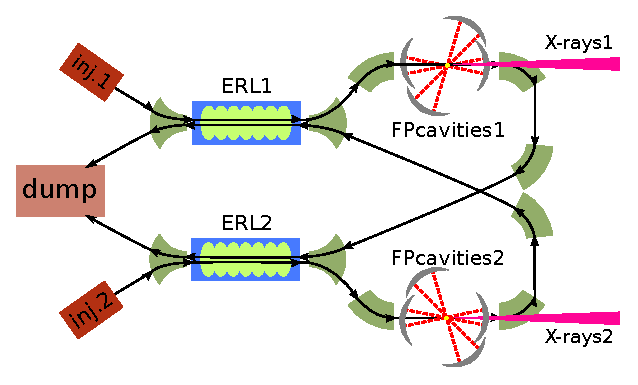
\includegraphics[width=0.9\linewidth]{images/BriXS.eps}
	\caption{Layout of BriXS, the MariX-ICS source: the energy recovery linacs accelerate the electrons to up to 300\,MeV, magnetic quadrupoles then guide the bunches to the Fabry-Perot cavities where X-Rays are produced. In each branch there are two crossed cavities in order to operate in dual-color mode.}
	\label{fig:brixs}
\end{figure}
BriXS is the name of the MariX inverse Compton scattering X-ray source, it is being developed with the aim of providing a synchrotron-like light source with limited footprint (laboratory-sized) and costs. His compactness and affordability will greatly benefit small research institutions and clinics, enabling innovative research and medical diagnosis and therapy.

BriXS radiation will be tunable in energy (20\,keV - 180\,keV), with a relative bandwidth of $\Delta E/E = 1-10\%$ and intensities  of $10^{11}-10^{13}$ photons/s. The beam will have a higher divergence than typical synchrotron light (10x10\,cm$^{2}$ at less than 100\,m from the interaction point), this is useful in medical application where uniformity and broadness of the light is required to allow single-shot imaging.
One of the key features of BriXS, and the main one addressed in this thesis, will be the production of X-rays with two different energies (``colors'') with a fast switch time between the two. Dual color X-rays can be used to probe matter in pump-probe experiments, but also to provide better biomedical imaging such as in K-edge color subtraction and microtomography \parencite{Jacobson1953}.
In pump and probe experiments one pulse (pump) is used to excite atoms in the sample to a higher energy state, while a different second pulse (probe) is used to study the atomic, electronic and magnetic structure of the sample.
K-edge subtraction (KES) imaging exploits the sudden change in the absorption coefficient of a contrast agent at a precise energy. An image is taken with X-rays just below the K-edge energy and then another with X-rays just above. The attenuation coefficient of the tissue doesn't vary much with energy, while that of the contrast agent changes sharply. By combining these two by logarithmic subtraction it is possible to produce hybrid images that highlight the contrast agent, while unwanted structures have their contrast reduced \parencite{Lehmann1981}. Both acquisition are made after the injection of the contrast agent and in temporal proximity to avoid patient/sample movement. The main clinical application of KES is today coronary angiography where iodine is used as the contrast agent thanks to its absorption edge at 33.17\,keV (see Fig \ref{fig:iodine}). Coronary angiography is extremely useful in cancer detection, in particular for breast cancer: in fact in some cases screening mammography proves ineffective in finding the tumor, while KES can easily identify the extra blood vessels formed around it \parencite{Lewin2003}. Having explained the importance of KES, the aim of this thesis is to develop the system that will enable BriXS to easily and swiftly shift between the two radiation energies. Since iodine contrast imaging is our objective, the radiation will be tailored to its K-edge energy, at 32 and 34\,keV.
\begin{figure}
	\centering
	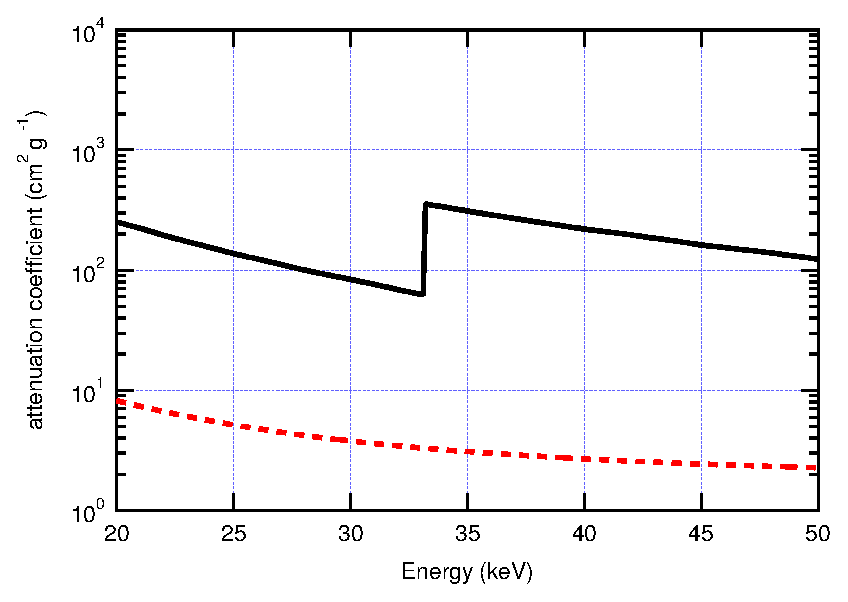
\includegraphics[width=0.9\linewidth]{images/iodine.eps}
	\caption{Linear attenuation coefficient as a function of photon energy. For iodine (solid black) a sharp absorption edge is present at 33.17\,keV, while it is absent for soft tissue (dashed red). Image is taken from \parencite{CDR}}
	\label{fig:iodine}
\end{figure}

Other applications of BriXS include Phase Contrast imaging, in which the sample internal structure is probed by measuring the phase shift it introduces on the radiation, radiotherapy, in particular breast cancer rotational radiotherapy which is now available only in a few centers in the world, X-ray fluorescence and diffraction experiments.

The structure of the BriXS facility is represented in Fig \ref{fig:brixs}, it has two symmetric beam lines in which electron bunches are produced in two injectors with repetition rate of 100\,MHz resulting in an average current of 20\,mA. The beams are then accelerated through two Energy Recovery Linacs (ERL) towards the interaction point (IP). Here the electrons interact with the photons inside two Fabry-Perot cavities (for a total of four cavities) and generate X-rays through inverse Compton scattering. The beams are then reinserted in the opposite ERL where they are decelerated and their energy recuperated. This coupled scheme permits to drive two independent Compton sources while simultaneously being more stable than a single ERL scheme.
The injectors for BriXS and the FEL and the Fabry-Perot cavities use the radiation produced by the Laser system, which includes Laser oscillators and cavities.

\section{The Laser system}
\begin{figure}
	\centering
	\includegraphics[width=1\linewidth]{images/pm.pdf}
	\caption{The MariX Laser system}
	\label{fig:photonic}
\end{figure}
Both MariX sources are driven by the Laser system, which uses a single laser oscillator as seed. The oscillator is mounted on an optical table, while the Fabry-Perot cavities are placed at the Interaction Points. The scheme also includes the fiber amplifiers, the temporal and spatial shaping system for the RF-guns, a Mach-Zender amplitude modulator, and two stabilization feedback systems.

The purpose of this optical system is to provide adequate radiation pulses in order to generate the electron bunches needed for both the FEL and the ICS source, but also to pump the optical cavities to the power necessary for the scattering process. Using a single laser source yields the advantage of having intrinsic synchronization between the laser pulses and the electron bunches. The light coming from the mode-locked pulsed laser is divided into three lines: one dedicated to the resonant cavities, one to the two RF-guns for the Compton source, and one to the RF-gun for the FEL. Each line will have a power of about 100\,mW before being amplified through multiple fiber amplifier stages. The repetition rate of the oscillator is 100\,MHz, in the FEL line it is reduced to 1\,MHz by the means of the Mach-Zender amplitude modulator.
Before entering the Fabry-Perot cavities the power is brought to about 200\,W, once inside the cavity the light pulses are superimposed with each other and the power reaches a value determined by the cavity Finesse, from 1000 to 10000 times the input power. In MariX we aim to obtain an enhancement factor of at least 2500, that is an average power of 500\,kW inside the cavity, and to possibly get to even higher figures.
The Compton RF-guns line is also amplified to 200\,W before being upshifted to the $4^{th}$ armonic by the means of two non-linear crystals. The pulse is then temporally and spatially shaped to achieve maximum efficiency in the photoelectric process. The FEL line is similar but the power is lower: about 1\,W at 1\,MHz, the pulse is also upshifted and shaped.

The cavities are stabilized against the laser using the Pound-Drever-Hall (PDH) technique \parencite{Black2001}, this is needed as the cavity electromagnetic modes needs to exactly match the oscillator modes. Another feedback system is used to synchronize the laser oscillator with an external reference.

\subsection{Laser oscillator}
A pulsed laser (as opposed to a continuous wave laser) is used in order to reach the high photon flux for the Compton process and the electronic bunches production. The oscillator of choice is a Yb-fiber mode-locked laser, delivering 100-200\,fs pulses\footnote{The oscillator in our laboratory has an in-built compressor to regulate the pulse length. Using an autocorrelator we measured a minimum pulse length of 130\,fs.} at 100\,MHz on a carrier wavelength of 1030\,nm. To reach maximum coupling with the Fabry-Perot cavities the laser beam must be single mode and have a spatial profile as similar to that of the cavity fundamental mode\footnote{Cavity modes theory will be dealt with in the next chapter.} (TEM$_{00}$) as possible, that is with a beam quality factor $M^2$ close to 1, where $M^2=1$ represents a perfectly gaussian intensity profile. Any mode non resonant in the cavity will not be coupled, that is reflected by the input mirror and its power wasted. Since we want the ICS source to be controllable in polarization we need it to have a high degree of polarization (close to  100\%), the source must also have good pointing stability and pulse to pulse stability. An Yitterbium-fiber laser meets this requirements: the fiber (which is also the gain medium) guides the beam propagation making it reach excellent spatial quality and simultaneously maintaining the beam polarization. The fiber can be pumped with laser diodes at 975\,nm with great quantum efficiency, reducing the power wasted into heat. This means that the system doesn't need extreme cooling and is compact.

To explain why the stabilization systems are needed we need to describe the mode-locked laser pulses in the temporal and spectral domain. In the time domain the pulses can be described by the oscillation at the carrier frequency $f_c$ and the periodic intensity envelope with period $T$. The phase shift between the two $\Delta\Phi_{CEO}$ is called carrier-envelope offset. In the frequency domain the pulses can be described by the repetition rate $f_{rep}=1/T$ and the $f_{CEO}=\Delta\Phi_{CEO} f_{rep}/2\pi$. The frequency comb is then:
\begin{align}
f_m = m f_{rep} + f_{CEO} = \left(m  + \frac{\Delta\Phi_{CEO}}{2\pi}\right) f_{rep}
\end{align}
To control the frequency comb a fine tuning of both $f_{rep}$ and $\Delta\Phi_{CEO}$ is necessary, the former to synchronize the laser with a reference and the latter to match the laser modes with the cavity modes.
The comb experiences fluctuations caused by pump and quantum noise, mechanical vibrations and nonlinear effects of the gain medium; the purpose of the two feedback stabilization systems is to compensate this fluctuations.

Oscillators with the requested characteristics are available on the market: both the Orange Menlo and the Origami One Five are candidates for the role. In our laboratory we currently use the Orange laser for R\&D purposes.

\begin{figure}
	\centering
	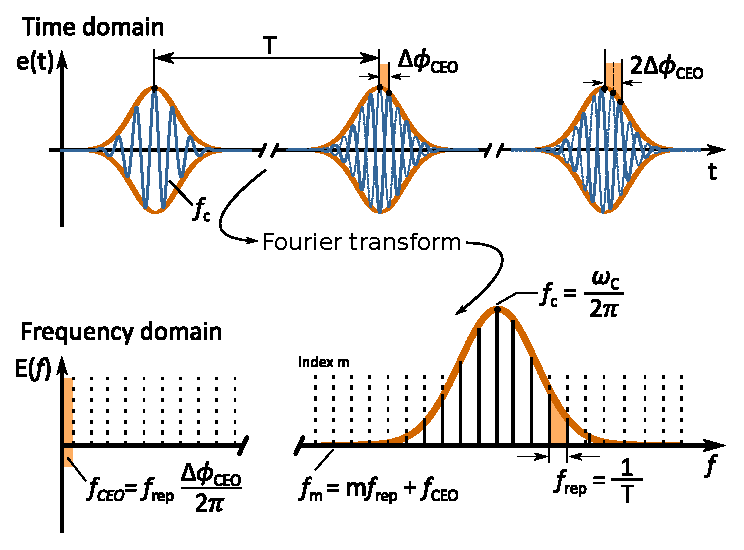
\includegraphics[width=0.9\linewidth]{images/comb.eps}
	\caption{Representation of a mode-locked laser pulse in the time domain and its frequency comb in the Fourier domain.}
	\label{fig:comb}
\end{figure}

\subsection{Fiber amplifiers}
To amplify the pulses to the requested power the Chirped-Pulse-Amplification (CPA) technique \parencite{Strickland1985} will be used\footnote{For developing the CPA technique, Donna Strickland and Gérard Mourou have been awarded the 2018 Nobel Prize in physics “for their method of generating high-intensity, ultra-short optical pulses”.}.
In this scheme the pulses are stretched temporally by introducing a linear chirp, delaying each frequency by a different amount. This reduces the maximum power of the pulse in order to avoid fiber damage and non-linear effects such as self-phase modulation (SPM) that can spoil the spatial quality of the beam.
\iffalse We can describe the electric field of a simple gaussian pulse as superposition of monochromatic waves. Since the Fourier transform of a gaussian curve is also gaussian we have:
\begin{align}
E(t) = \mathrm{e}^{-\frac{\omega^2}{\sigma^2}} \mathrm{e}^{i\omega t}
\end{align}
To introduce a linear chirp we make the substitution $t\rightarrow t-\alpha\omega$:
\begin{align}
E(t) = \mathrm{e}^{-\frac{\omega^2}{\sigma^2}} \mathrm{e}^{i\omega (t-\alpha\omega)} = \mathrm{e}^{-\frac{\omega^2}{\sigma^2}} \mathrm{e}^{-i\alpha\omega^2} \mathrm{e}^{i\omega t}
\end{align}
\fi
The stretching of the pulse can be achieved with chirped volume Bragg gratings (CVBG), which are diffraction gratings engraved into a monolithic crystal that reflect different wavelengths at different positions, as represented in Fig \ref{fig:CVBG}.
\begin{figure}
	\centering
	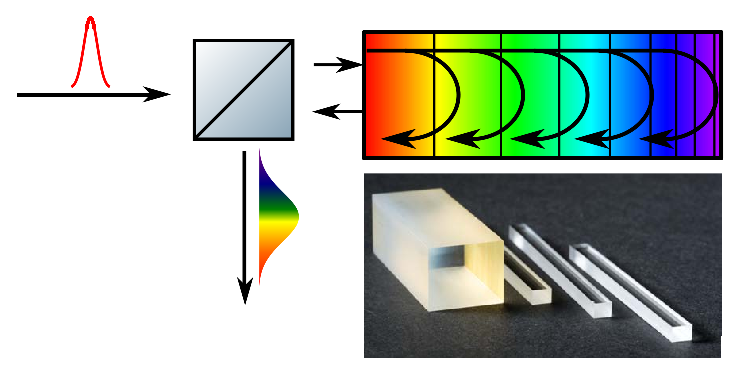
\includegraphics[width=0.9\linewidth]{images/CVBG.eps}
	\caption{Chirped Volume Bragg Grating: a short laser pulse that enters a CVBG is stretched as its spectral components are delayed differently depending on the frequency. Another CVBG can be used to compress the pulse to its original length after amplification. CVBG are engraved into monolithic crystals as displayed in the lower picture.}
	\label{fig:CVBG}
\end{figure}
The chirped pulse is then coupled in a large mode area (LMA) polarization maintaining double clad fiber. The fiber is composed by a single mode Yb-doped inner core (the gain medium) in which the pulse to be amplified is coupled, and a larger multi-mode cladding in which the laser pump is launched. By coupling the pump in a larger area than the seed nonlinear effects and fiber damage are avoided, in addition the pump source doesn't need to be single mode and can be launched efficiently thanks to a big numerical aperture \parencite{Paschotta1997}. The Yb-doped fiber allows up to 7\,dB/m amplification at a pump wavelenght of 975\,nm, with a typical conversion efficiency of 60\%.
The amplified pulses are then compressed with another CVBG, reducing the chirp to reach the desired pulse length; in our Compton source we need a pulse length of a few ps (to match that of the electron bunch) while for the RF-Guns tens of ps are required.
\begin{figure}
	\centering
	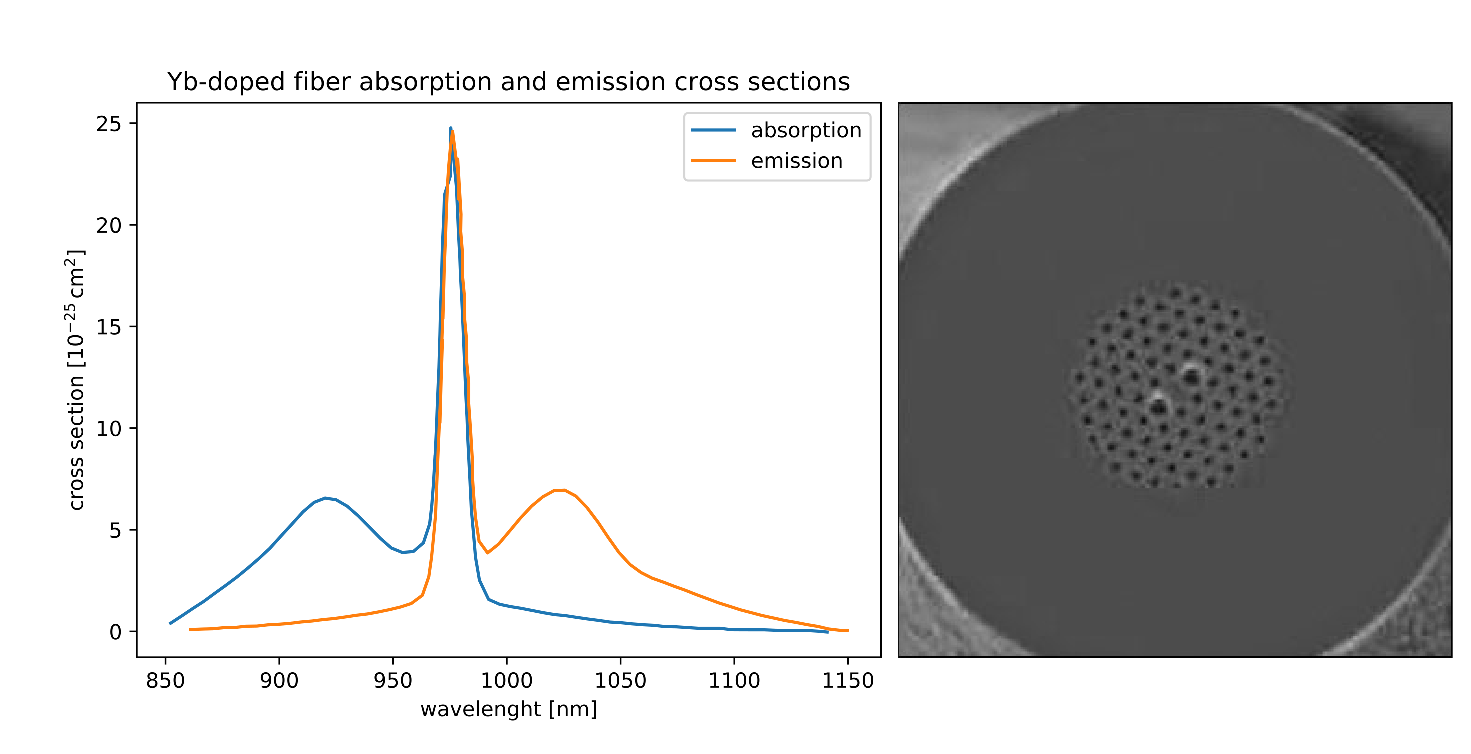
\includegraphics[width=0.9\linewidth]{images/ybfiber.eps}
	\caption{On the left: typical absorption and emission cross sections for a Yb-doped fiber. The large emission spectrum makes it ideal for ultra-short pulse amplification, maximum pump efficiency is reached at 975\,nm. On the right: a Photonic Crystal Fiber (PCF), in these fibers the index of refraction in the cladding is modified by small air cavities, confining the seed beam in the small core. The PANDA stress rods (the two dots at the center) make the fiber Polarization Maintaining. Picture and data from Thorlabs, Inc.}
	\label{fig:ybfiber}
\end{figure}

The amplifier scheme will be composed of three stages, as different powers need different fiber dimensions and cooling systems. Multiple stages are also needed to reduce noise sources such as SPM and amplified spontaneous emission (ASE). Self-phase modulation arise in fibers when the intensity of the pulse is high because of the Kerr effect, that is the dependence of the refractive index of the medium from the square of the electric field. It can lead to frequency broadening and pulse spreading \parencite{Stolen1978}, but also to bad coupling with the Fabry-Perot cavities modes. Amplified spontaneous emission occurs when the power is low but the gain is high (30-40\,dB according to \parencite{Paschotta1997}) and reduces the total gain while introducing unwanted noise. 
In the cavities and Compton lines, the first stage will bring the 100\,mW seed to about 2\,W, the second will reach 60\,W and the last one will get to 200\,W. Since the first stage has high gain a forward pumping scheme will be used to reduce the effect of ASE \parencite{Paschotta1997}, with the seed and pump beam entering the fiber from the same side. The other stages will instead use a backward pumping scheme to reduce the nonlinear effects in the fiber due to the high power. The two schemes yield the same output power, but in the backward case the average power inside the fiber is lower. While a commercial solution for the first stage is available, the other two stages will be developed in the R\&D phase.

\subsection{Fabry-Perot cavities}
\begin{figure}
	\centering
	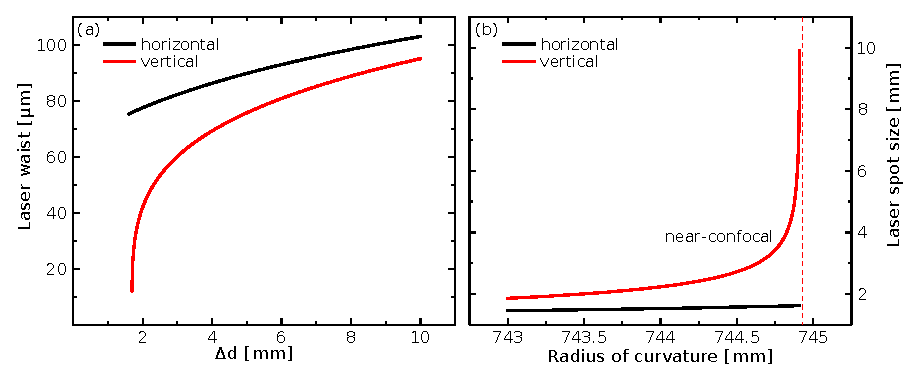
\includegraphics[width=0.9\linewidth]{images/waistspot.eps}
	\caption{(a) The laser beam spot size at the waist as a function of the distance between the curved mirrors. (b) The spot size at the mirror surface as a function of the mirrors radius of curvature.}
	\label{fig:waistspot}
\end{figure}
To reach the high photon flux needed for the Compton process a Fabry-Perot optical cavity can be used.
In an optical cavity the electromagnetic field can exist in stationary states called modes. Modes have well-defined wavelength and spatial profiles that must be matched to couple an external laser beam to a cavity. In the case of a pulsed laser the temporal matching condition must also be met, that is an incoming pulse must exactly overlap with the pulse resonating in the cavity. In the frequency domain this condition means that the pulse spectral comb must match the cavity spectral comb. After each round trip the intensity of the pulse inside the cavity increases until equilibrium is reached between gain and losses. The temporal condition fixes the cavity length to the inverse of the repetition rate of the laser multiplied by the speed of light (or a multiple of this quantity):
\begin{align}
L = m \frac{c}{f_{rep}}
\end{align}
In our case we want a single pulse inside the cavity to achieve maximum peak power ($m=1$):
\begin{align}
L = \frac{c}{f_{rep}} \approx \frac{3*10^8\,\mathrm{m/s}}{100\,\mathrm{MHz}} = 3\,\mathrm{m}
\end{align}
\begin{figure}
	\centering
	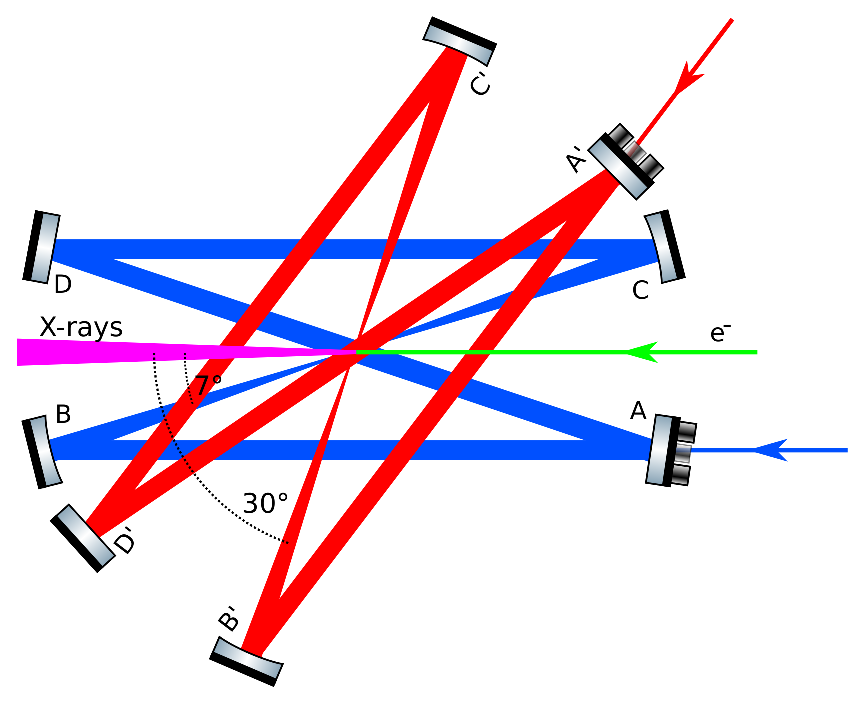
\includegraphics[width=0.9\linewidth]{images/doublecavity.eps}
	\caption{Scheme of the two 4-mirrors bow-tie confocal optical resonators. A and A' are the input couplers; B, B', C, C' are the curved mirrors and the distance between them regulates the spot size at the beam waist; D and D' are flat mirrors and are used to restore the cavities length when changing the distance between the curved mirrors.}
	\label{fig:bowtie}
\end{figure}
The cavity design of choice is a 4-mirrors (2 flat and 2 curved) bow-tie near-confocal cavity. This geometry has the advantage of being stable while also allowing adjustments of the beam waist without changing the length (which influences the resonant frequency) and vice-versa. In a Compton source fine tuning of the beam waist is necessary to better match the electron beam profile at the interaction point, which corresponds to the focus of the cavity. Changing the curved mirrors distance and restoring the length with the flat mirrors also allows to change the laser spot size on the mirrors: a big spot size is desired to avoid thermal deformation of the reflecting surface.

As it will be explained in the next chapter, the frequency of the X-rays produced through inverse Compton scattering presents a strong dependence from the angle between the interacting photons and electrons. We then propose to use two identical crossed Fabry-Perot cavities at two different angles in order to implement the ``dual color mode'', a key feature of BriXS. As represented in Fig \ref{fig:bowtie}, the electrons will pass between two of the first cavity mirrors, interacting with the pulse coming from mirror B at an angle of about 7\degree. To switch from one cavity to the other, we propose to use piezo-electric driven moving mirrors that can move the laser beam in and out of the interaction point. During the switch, the moving mirrors will translate the focus of the first cavity away from the electron beam while simultaneously placing the focus of the second cavity in the interaction zone. The angle of incidence with the second cavity will be about 30\degree, the two angles are chosen in order to bracket the iodine K-edge energy at 32 and 34\,keV. A key point is the fact that the two cavities must remains stabilized (in resonance with the oscillator) during the movement, in the third chapter I will present the experimental results we obtained which indicate that it is possible to switch between the two cavities without losing the matching and coupling with the external laser mode.

\subsection{4th armonic generation}
\begin{figure}
	\centering
	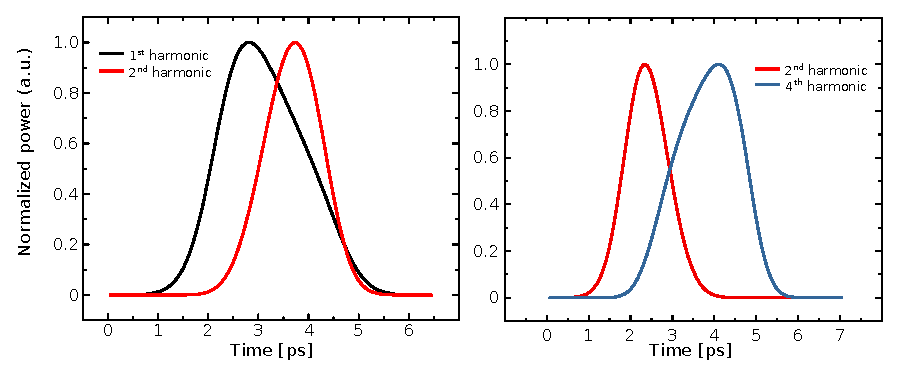
\includegraphics[width=0.9\linewidth]{images/harmonic.eps}
	\caption{Simulation of second and fourth harmonic generation in nonlinear birefringent crystals (LBO and CLBO). The resulting pulse length depend on the length of the crystal.}
	\label{fig:harmonic}
\end{figure}
High electron beam current and brightness require photocathodes with high Quantum Efficiency (QE). The natural choice is then to use semiconductor cathodes that have good QE in the UHV region. To get UHV light from the 1030\,nm pulses 4th harmonic generation through two nonlinear birefringent crystals will be employed, each doubling the frequency of the beam. The 2nd harmonic (515\,nm) will be produced inside a Lithium triborate (LBO, LiB$_3$O$_5$) crystal while the 4th harmonic (257.5\,nm) generation will take place in a Cesium Lithium Borate (CLBO, CsLiB$_6$O$_10$) crystal. Second harmonic generation (SHG) can be achieved when the so-called phase-matching condition is met: since the crystals are nonlinear an incoming field oscillating at $\omega$ will make the polarization oscillate at $2\omega$, if the two waves propagate at the same phase velocity oscillations generated at different places will interfere constructively and result in a $2\omega$ radiation field exiting the other end of the crystal. The phase-matching condition is then:
\begin{align}
n(\omega) = n(2\omega)
\end{align}
This condition is achievable in birefringent materials, that have different indexes of refraction for different field polarization. LBO and CLBO are uniaxial crystals, meaning they have index $n_o$ along two axes and an index $n_e$ along the third. In LBO the noncritical phase-matching can be used since $n_e$ presents a strong dependence on the temperature $T$, if the crystal is kept at a temperature such that $n_o(\omega) = n_e(2\omega,T)$ SHG will take place. In CLBO critical phase-matching can be used instead. If the second harmonic travels at an angle $\theta$ with respect to the crystal axis, it will travel with an index of refraction given by:
\begin{align}
\frac{1}{n^2(2\omega,\theta)} = \frac{\sin^2\theta}{n^2_o(2\omega,\theta)} + \frac{\cos^2\theta}{n^2_e(2\omega,\theta)}
\end{align}
Then for a particular angle the phase-matching condition $n_o(\omega)=n(2\omega,\theta)$ can be satisfied. In this case the extraordinary beam experience walk-off, this effect can be mitigated using two CLBO crystal glued together with opposing orientation. Simulation on the crystals effect on the pulse length are shown in Fig \ref{fig:harmonic}.

\subsection{Temporal shaping}
\begin{figure}
	\centering
	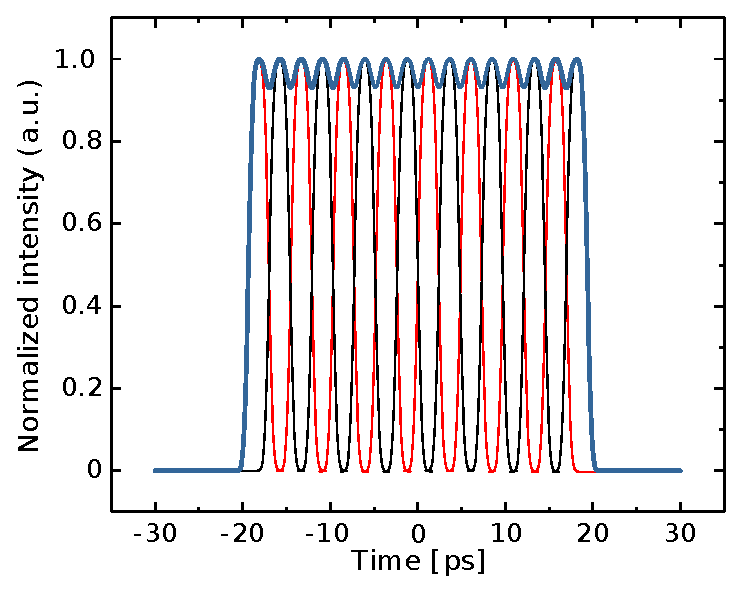
\includegraphics[width=0.9\linewidth]{images/temporal.eps}
	\caption{In this simulation a $\sim$2\,ps pulse is shaped by four $\alpha$-BBO crystals of lengths 22, 11, 5.5, 2.75 nm to get to the 40\,ps figure necessary for the FEL line. Red and black indicate orthogonal polarizations while blue is the sum of the two.}
	\label{fig:temporal}
\end{figure}
To optimize the temporal profile of the pulse for the photoemission process the passive pulse stacking technique can be used. This consists in overlapping replicas of the original pulse to obtain a rectangular-shape pulse and it can be done either with delay lines or with a set of birefringent crystals such as Barium beta borate ($\alpha$-BBO). Since in such a crystal we have two different group velocities for horizontal and vertical polarization, a pulse linearly polarized at 45 degrees will divide in two equal intensity replicas having opposite polarization, with a time separation between the two
\begin{align}
t_d = \frac{1}{c} \left|n_{g,o}L-n_{g,e}L\right|
\end{align}
With $n_g=c\,\partial k/\partial \omega$ being the group refractive index for the two polarizations and $L$ the crystal length.
Further replicas can be obtained adding a second crystal of length $L/2$ and so on until the pulse has the desired length and shape. For the Compton line a pulse of $\sim$20\,ps is desired while for the FEL line $\sim$40\,ps. Since the pulse length is estimated to be 1.6\,ps after the amplification and 4th harmonic generation system a set of three crystals can be used for the Compton line and four for the FEL.

\subsection{Spatial shaping}
\begin{figure}
	\centering
	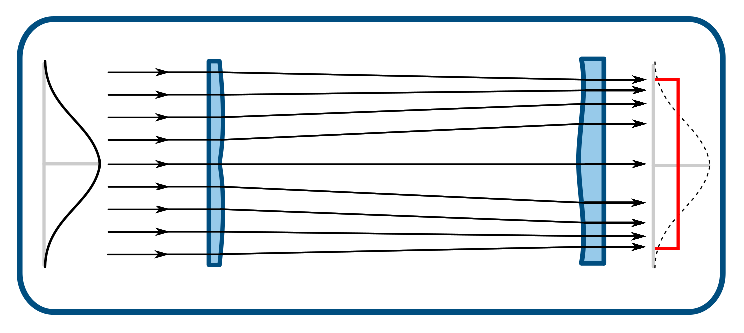
\includegraphics[width=0.9\linewidth]{images/pishaper.eps}
	\caption{$\pi$-shaper: two aspherical lenses can transform a gaussian spatial profile into a flat-top profile.}
	\label{fig:pishaper}
\end{figure}
The intensity profile of the beam can be modified with a set of two aspherical lenses, in particular a commercially available $\pi$-shaper can modify a gaussian beam into a flat-top beam.
Since such a beam is not a free-space mode, i.e. its profile is not maintained in free-space propagation, a telescopic system must be used to reproduce its rectangular profile on the photocathode.
\begin{figure}
	\centering
	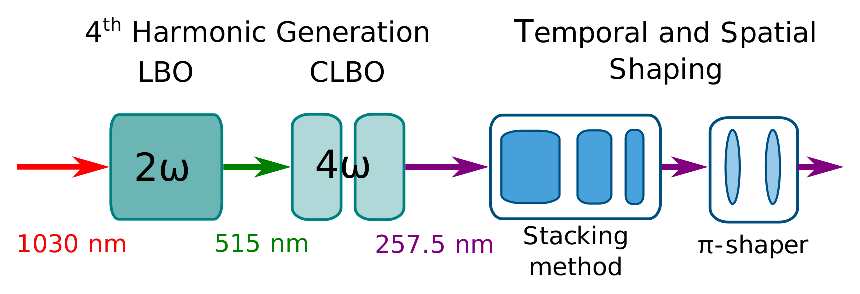
\includegraphics[width=0.9\linewidth]{images/rfgun.eps}
	\caption{Transformation of the pulse for the RF-guns line: firstly two second harmonic generation stages bring the wavelength to 257.5\,nm, then temporal and spatial shaping modify the pulse longitudinal and transverse profile to optimize the photoemission process.}
	\label{fig:rfgun}
\end{figure}

\subsection{Mach-Zender amplitude modulator}
\begin{figure}
	\centering
	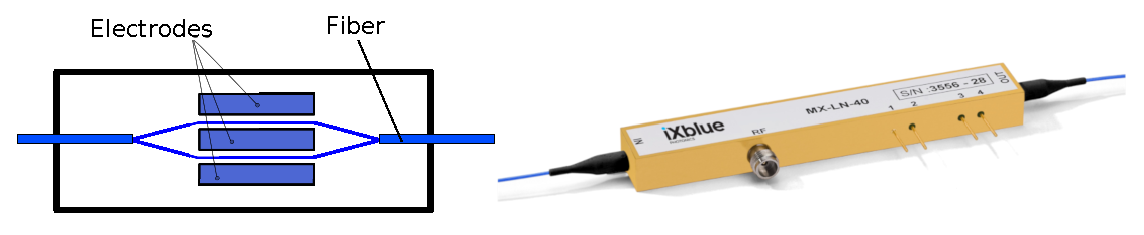
\includegraphics[width=0.9\linewidth]{images/mach.eps}
	\caption{Example of a Mach-Zender amplitude modulator.}
	\label{fig:mach}
\end{figure}
The FEL RF-guns line requires the electron bunches to have a repetition rate of 1\,MHz. Since we want to use the 100\,MHz laser oscillator to drive the entirety of the Laser system, a Mach-Zender amplitude modulator con be used to reduce the repetition rate to the desired level. Such a modulator is in fact an interferometer that can introduce a phase difference between the two paths, leading to constructive of destructive interference. To change the relative phase materials like Lithium niobate (LiNbO$_3$), which has a refractive index strongly dependent on the applied electric field, can be used. By applying an electric field with the right intensity and timing only 1 every 100 pulses exits the interferometer.

\subsection{Stabilization systems}
In order for the laser oscillator to have a stable repetition rate $f_{rep}$ it needs to be synchronized with an external radio-frequency source or with an optical source. The time jitter is about 150\,fs for the former solution and a few fs for the latter. Such solutions are commercially available and an example is shown in Fig \ref{fig:synchro}.
\begin{figure}
	\centering
	\includegraphics[width=0.9\linewidth]{images/synchro.eps}
	\caption{Scheme and picture of the synchronization module for the Orange Menlo laser by Menlo Company. It generates an error signal comparing the phase difference with the laser and acts on the oscillator with two actuators: a piezo and a mechanical stage.}
	\label{fig:synchro}
\end{figure}

The other stabilization system deals with the mode matching between the cavity and the laser source. Thermal effects and mechanical noise modify the length of the cavity that needs real-time correction, but also source noise must be corrected.
We recall that the frequency comb of the oscillator is:
\begin{align*}
f_m = m f_{rep} + f_{CEO}
\end{align*}
while that of the cavity is:
\begin{align}
f_{cm} = m f_{FSR}
\end{align}
where $f_{FSR} = c/L$ is the Free Spectral Range of the cavity, that is the distance in frequency between two TEM$_{00}$ modes of the cavity and depends only on the cavity length.
The matching condition for a mode identified by the index $m_0$ is then:
\begin{align}
m_0 f_{rep} + f_{CEO} = m_0 f_{FSR}
\end{align}
From which is clear that fine stabilization of the cavity length is needed to maintain $f_{FSR} = f_{rep} + f_{CEO}/m_0$. A typical value for $m_0$ would be $L/\lambda = 3\times10^6$.
For a mode-locked laser, the pulse is composed of several modes separated by $f_{rep}$, let's calculate the frequency difference between $f_m$ and $f_{cm}$ when $m=m_0+\delta m$:
\begin{align}
\delta f &= (m_0+\delta m)(f_{rep} + f_{CEO}/m_0) - ((m_0+\delta m) f_{rep} + f_{CEO})\\
\delta f &= f_{CEO}\frac{\delta m}{m_0}
\end{align}
Since all the modes in the pulse should match a cavity mode $f_{CEO}$ should be kept as low as possible, ideally at 0. To control both $f_{FSR}$ and $f_{CEO}$ a double PDH \parencite{Black2001} system can be used, as shown in Fig \ref{fig:PDH}. The first PDH system generates an error signal looking at the phase difference between the resonant mode transmitted and reflected by the cavity and two non resonant sidebands completely reflected. The second system only looks at a tiny portion of the reflected spectrum in order to highlight the frequency difference caused by the $f_{CEO}$. Both signals are fed in a Proportional-Integral-Derivative servo that drives actuators both in the cavity (a piezo) and in the laser source (controlling the pump current). The first PDH system has been successfully implemented in our laboratory and can stabilize our prototype cavities.
\begin{figure}
	\centering
	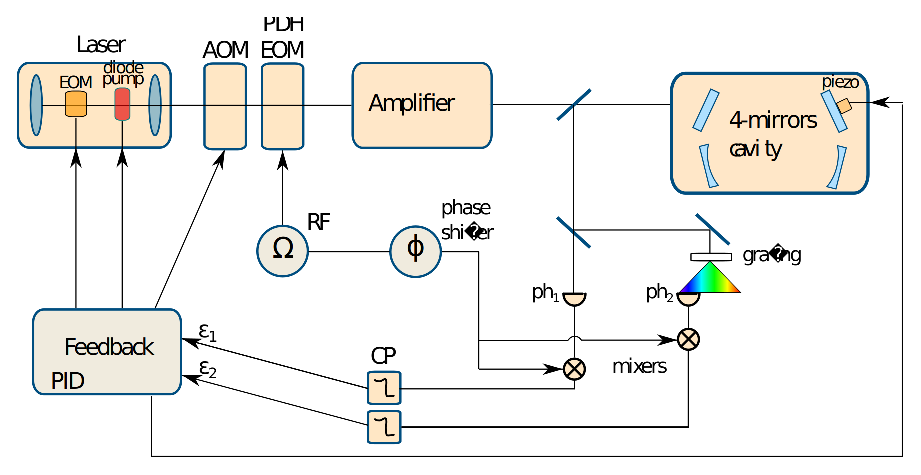
\includegraphics[width=0.9\linewidth]{images/PDH.eps}
	\caption{The double PDH system used to stabilize the cavity against the laser oscillator.}
	\label{fig:PDH}
\end{figure}